% !TEX root = ./Basilisk-opNavPoint-20180427.tex

\section{Model Description}

\begin{figure}[t]
	\centerline{
		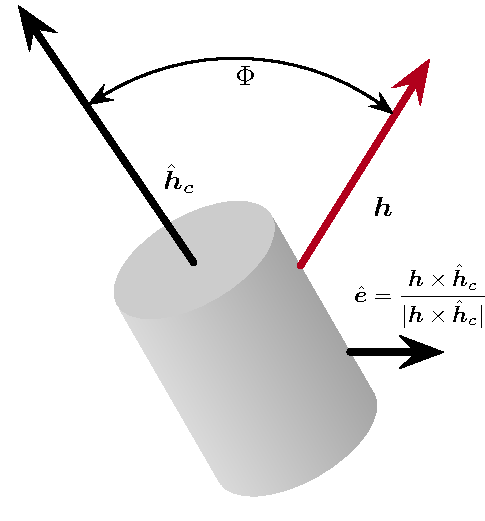
\includegraphics{Figures/Heading}
	}
	\caption{Body Vector Illustrations.}
	\label{fig:Fig1}
\end{figure}

\subsection{Module Goal}
This attitude guidance module has the goal of aligning a commanded camera-fixed spacecraft vector $\hat{\bm h}_{c}$ with another input vector $\bm h$.  If $\hat{\bm h}_{c}$ is the camera boresight, this module will compute the attitude tracking errors to align the camera towards the target, i.e. achieve relative pointing. 

Besides $\bm h$, the second input vector is the inertial body angular velocity vector $\bm\omega_{B/N}$. As the desired planet pointing orientation is unknown, the inertial reference frame acceleration $\dot{\bm\omega}_{R/N}$ is set to zero,.  

Note that this module does not establish a unique target-pointing reference frame.  Rather, it simply aligns $\hat{\bm h}_{c}$ with $\bm h$ which is an under-determined 2 degree of freedom condition.  Thus, the rotation angle about $\bm h$ is left to be arbitrary in this planet pointing module. 

\subsection{Equations}
\subsubsection{Good Planet Direction Vector Case}\label{sec:withHeading}
In the following mathematical developments all vectors are assumed to be taken with respect to a camera-fixed frame $\cal C$.  The attitude of the camera relative to the target reference frame $\cal R$ is written as a principal rotation from $\cal R$ to $\cal C$. The target $\cal R$ is defined simply by the vector $\hat{\bm h}_{c}$ and body frame vectors. Thus, the associated principal rotation vector $\hat{\bm e}$ is
\begin{equation}
	\label{eq:ssp:1}
	\hat{\bm e} = \frac{\bm h \times \hat{\bm h}_{c}}{|\bm h \times \hat{\bm h}_{c}|}
\end{equation}
Note that the planet direction vector $\bm h$ does not have to be a normalized input vector.  

The principal rotation angle between the two vectors is given through
\begin{equation}
	\label{eq:ssp:2}
	\Phi = \arccos \left( \frac{\bm h  \cdot \hat{\bm h}_{c} }{|\bm h|} \right)
\end{equation}

Next, this rotation from $\cal R$ to $\cal C$ is written as a set of MRPs through
\begin{equation}
	\label{eq:ssp:3}
	\bm\sigma_{C/R} = \tan\left(\frac{\Phi}{4}\right) \hat{\bm e}
\end{equation}
The set $\bm\sigma_{C/R}$ is the attitude error of the output attitude guidance message.  

While the attitude errors are tracked in the camera frame, the rates are tracked in the body frame. This can be done since the camera is fixed in the body frame.
The module allows for a nominal spin rate about the planet heading axis by specifying the module parameter {\tt planetAxisSpinRate} called $\dot \theta$ in this description.  The nominal spin rate is thus given by
\begin{equation}
	\leftexp{B}{\bm\omega}_{R/N} = [\cal B \cal C]\leftexp{C}{\hat{\bm h}} \dot\theta
\end{equation}
Note that this constant nominal spin is only for the case where the planet is visible and the planet-heading vector measurement is available. 

If the spacecraft is to be brought to rest, $\bm\omega_{R/N} = \bm 0$, then $\dot\theta$ should be set to zero.  The tracking error angular velocity vector is computed using:
\begin{equation}
	\label{eq:ssp:4}
	\bm\omega_{B/R} = \bm\omega_{B/N} - \bm\omega_{R/N}
\end{equation}

Finally, the attitude guidance message must specify the inertial reference frame  acceleration vector.  This is set to zero as the roll about the planet heading is assumed to have a constant magnitude and inertial heading.
\begin{equation}
	\dot{\bm \omega}_{R/N} = \bm 0
\end{equation}

\subsubsection{No planet Direction Vector Case}
 If $\Phi$ is less then the module parameter {\tt minUnitMag}, it is assumed that no good planet heading vector is available and the attitude tracking error $\bm\sigma_{C/R}$ is set to zero.   
 
 Further, if the planet is not visible, the module allows for a non-zero body rate to be prescribed.  This allows the spacecraft to engage in a constant rate tumble specified through the module configuration vector {\tt omega\_RN\_B}.  In this case, the tracking error rate is evaluated through
 \begin{equation}
 	\label{eq:ssp:6}
	\bm\omega_{B/R} = \bm\omega_{B/N} - \bm\omega_{R/N}
 \end{equation}
 and the output message reference rate is set equal to the prescribed $\bm\omega_{R/N}$ while the reference acceleration vector $\dot{\bm \omega}_{R/N}$ is set to zero.

 
 \subsubsection{Collinear Commanded and Planet Heading Vectors}
First consider the case where $\bm h \approx \hat{\bm h}_{c}$.  In this case, the cross product in Eq.~\eqref{eq:ssp:1} is not well defined.  Let $\epsilon$ be a pre-determined small angle.  Then, if $\Phi < \epsilon$, the attitude tracking error is set to $\bm\sigma_{C/R} = \bm 0$.
 
However, if $\bm h \approx -\hat{\bm h}_{c}$, then an eigen-axis $\hat{\bm e}$ that is orthogonal to $\hat{\bm h}_{c}$ must be determined.  Let the body frame be defined through \frameDefinition{B}.  The eigen-axis is determined first by taking a cross product with $\hat{\bm b}_{1}$:
 \begin{equation}
	\label{eq:ssp:7}
	\hat{\bm e}_{180} = \frac{ \hat{\bm h}_{c} \times \hat{\bm b}_{1}}{| \hat{\bm h}_{c} \times \hat{\bm b}_{1}|}
\end{equation}
If $\hat{\bm h}_{c} \approx \hat{\bm b}_{1}$, then this $\hat{\bm e}$ vector will have a small norm.  In this ill-determined case, the $\hat{\bm e}$ vector is determined using
 \begin{equation}
	\label{eq:ssp:8}
	\hat{\bm e}_{180} = \frac{ \hat{\bm h}_{c} \times \hat{\bm b}_{2}}{| \hat{\bm h}_{c} \times \hat{\bm b}_{2}|}
\end{equation}
As $ \hat{\bm h}_{c}$ cannot be aligned with both $\hat{\bm b}_{1}$ and $\hat{\bm b}_{2}$, this algorithm determines a unique eigen axis $\hat{\bm e}_{180}$ for the case that the principal rotation angle is close to 180 degrees, or $\pi - \Phi < \epsilon$.  This special case eigen axis is only computed once in the module reset routine.

In this scenario the angular velocity tracking error is evaluated using the same method as outlined in section~\ref{sec:withHeading}.
 
 